\section{M/M/1/K queue}
    We devised a simple Erlang system that can act as a simple M/M/1/K.
    \paragraph{Why M/M/1/K?} An average component in a distributed system can be modeled as an M/M/1/K, due to the exponential inter-arrival rate of messages, the exponential distribution of the execution delay and the message buffer size of a component.

    The system has two components \texttt{worker\_1}, \texttt{worker\_2}, the components are made of a buffer queue of size $K$ and a worker process.
    
    The system sends $n$ messages per second following a Poisson distribution to \texttt{worker\_1}'s queue, the queue then reduces its available buffer size. \\
    
    The buffer notifies its worker, which then does $N$ loops, which are defined upon start, of fictional work. The worker then passes a message to \texttt{worker\_2}'s queue, which has another queue of same size, who passes the message to \texttt{worker\_2}'s worker, which does the same amount of loops. When a worker completes its work, it notifies the queue, freeing one "message" from its buffer size. \\
    
    If the queue's buffer is overloaded, it will drop the incoming message and consider the execution a failure. \\
    
    A probe $p$ is defined, which observes the execution from when the first message up until \texttt{worker\_2} is done.
    \begin{figure}[H]
        \begin{center}
            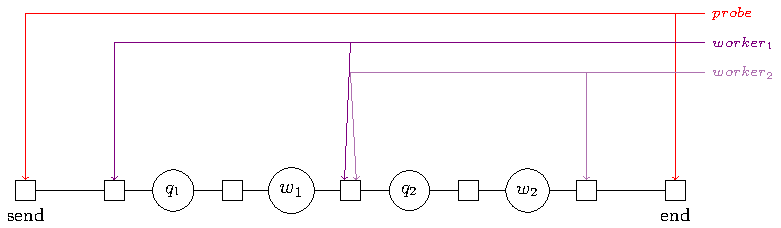
\includegraphics[scale=1.2, width=\textwidth]{tikz/mm1k.pdf} 
        \end{center}
        \caption{Outcome diagram of the M/M/1/K queue}
    \end{figure}

    \subsection{Determining parameters dynamically}
        We stated previously that determining parameters is something that must be done with an underlying knowledge of the system. The oscilloscope can provide knowledge of the system, here is an example of worker\_1 and worker\_2 as observed in the oscilloscope.

        Imagine the engineer supposes the workers executions should take around 6.5 ms to complete, but doesn't actually know how long the executions should take. The engineer, after having set the required parameters observes in the following graph in the oscilloscope \ref{fig:w1w2}.

    The oscilloscope shows the engineer that their assumptions do not correspond to the actual system $\Delta$Q, the user can then modify the parameters to observe the actual system's behaviour. By setting $dmax$ to 25 ms, he can observe the worker's $\Delta$Qs approaching 1.

\begin{figure}[H]
            \centering
            \begin{subfigure}{.5\textwidth}
                \centering
                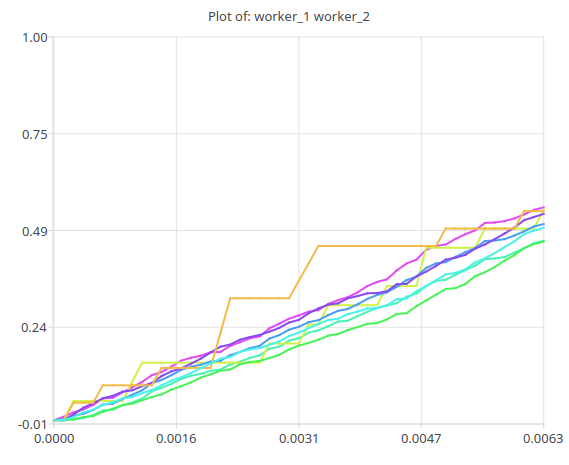
\includegraphics[width=0.98\textwidth]{img/w1w2.png}
                \label{fig:w1w2}
                \subcaption{worker\_1 and worker\_2 $\Delta$Qs plot with 6.5 ms $dMax$.}
            \end{subfigure}%
            \begin{subfigure}{.5\textwidth}
                \centering
                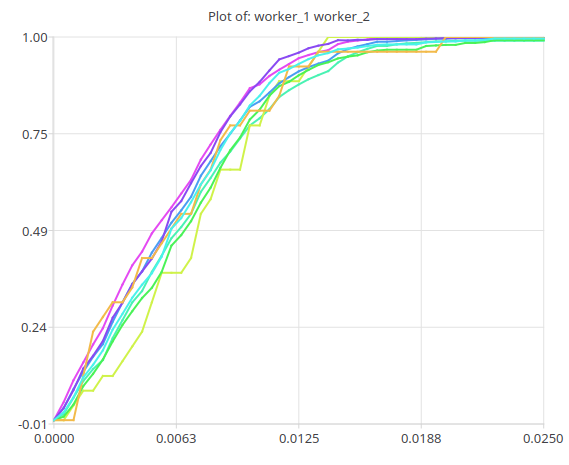
\includegraphics[width =0.98\textwidth]{img/w1w2hb.png}
                \label{fig:sub2}
                \subcaption{worker\_1 and worker\_2 $\Delta$Qs plot with 25 ms $dMax$} 
            \end{subfigure}
            \label{fig:w1w2hb}
            \end{figure}


    On the other hand, the engineer's assumption could have been what he truly expected from the system, in this case, the oscilloscope tells him that the system is not behaving as expected. 

    \paragraph{Low Load}

    At low load, we can observe in the oscilloscope how worker\_1 and worker\_2 mean $\Delta$Qs overlap. This is expected, even under overload or dependency conditions, worker\_1 and worker\_2 should have the same $\Delta$Qs.

If the system is not showing dependent behaviour, the probe \textbf{observed $\Delta$Q} and \textbf{calculated $\Delta$Q} should overlap. We can observe that in the graph below, as the mean CDF of both $\Delta$Qs overlap.



\begin{figure}[H]
            \centering
            \begin{subfigure}{.5\textwidth}
                \centering
                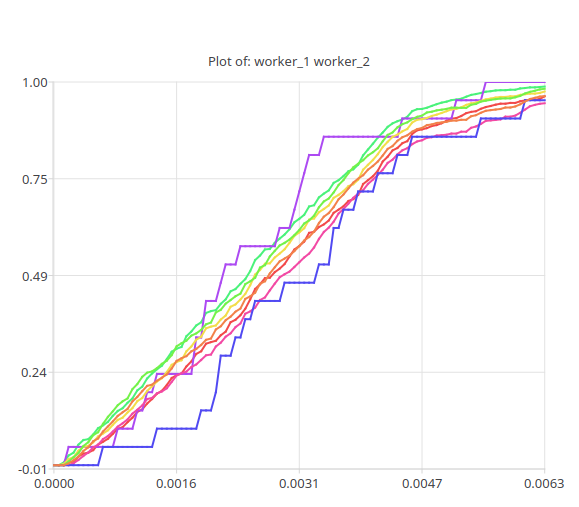
\includegraphics[width=0.98\textwidth]{img/superp21.png}
                \label{fig:sp21}
                \subcaption{worker\_1 (blue) and worker\_2 (purple) $\Delta$Q plots as shown in the oscilloscope}
            \end{subfigure}%
            \begin{subfigure}{.5\textwidth}
                \centering
                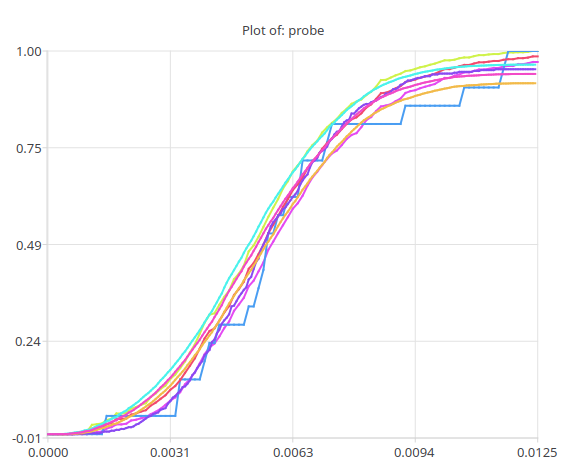
\includegraphics[width =0.98\textwidth]{img/superp22.png}
                \label{fig:sub2}
                \subcaption{probe $\Delta$Q plots as shown in the oscilloscope} 
            \end{subfigure}
            \label{fig:sp22}
            \end{figure}

\paragraph{Early signs of overload}
    
    Once the system is approaching overload, we can see the two means starting to diverge. As shown in a previous chapter, the observed (1) $\Delta$Q of the probe is below the calculated (2) $\Delta$Q. (explain better) 
    \begin{figure}[H]
        \begin{center}
            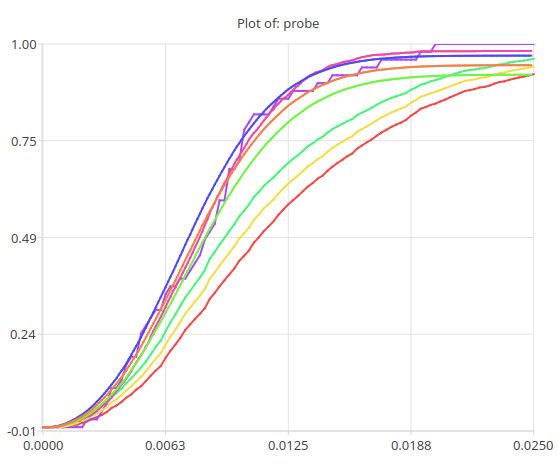
\includegraphics[scale=0.6]{img/diverging11.png}
        \end{center}
    \end{figure}
